%! Tex program = xelatex
\documentclass{article}
%中文
\usepackage[UTF8]{ctex}
%数学公式
\usepackage{amsmath,amssymb}
%\usepackage{ntheorem}
\usepackage{mdframed} %公式框1
% e.g., \newmdtheoremenv{theorem}{Theorem}
\usepackage{amsthm}
%边界
\usepackage[letterpaper,top=1cm,bottom=1.5cm,left=3cm,right=3cm,marginparwidth=1.75cm]{geometry}%table package
%Table
\usepackage{multirow,booktabs}
\usepackage{makecell}
%字体颜色
\usepackage{color}
\usepackage[dvipsnames]{xcolor}  % 更全的色系
%代码
\usepackage[OT1]{fontenc}
% MATLAB 代码风格
%\usepackage[framed,numbered,autolinebreaks,useliterate]{/Users/anye_zhenhaoyu/Desktop/Latex/mcode}
\usepackage{listings}
\usepackage{algorithm}
\usepackage{algorithmic}
\usepackage{pythonhighlight} % Python
%插图
\usepackage{graphicx}
%改变item格式
\usepackage{enumerate}
%物理
\usepackage{physics}
%extra arrows
\usepackage{extarrows}
% caption(居中指令)
%\usepackage[justification=centering]{caption}
\usepackage{caption}
% htpb
\usepackage{stfloats}
% pdf 拼接
\usepackage{pdfpages}
% 超链接url
\usepackage{url}

\def\RR{\mathbb{R}}
\def\ZZ{\mathbb{Z}}
\def\EE{\mathbb{E}}

\def\Trsp#1{#1^{\mathcal{T}}}
\def\LT{\mathcal{L}}

\def\bold#1{\boldsymbol{#1}}
\def\bw{\boldsymbol{\omega}}
\def\ba{\boldsymbol{a}}
\def\bb{\boldsymbol{b}}
\def\bc{\boldsymbol{c}}
\def\bd{\boldsymbol{d}}
\def\be{\boldsymbol{e}}
\def\bf{\boldsymbol{f}}
\def\bg{\boldsymbol{g}}
\def\bh{\boldsymbol{h}}
\def\bt{\boldsymbol{t}}
\def\bu{\boldsymbol{u}}
\def\bv{\boldsymbol{v}}
\def\bx{\boldsymbol{x}}
\def\by{\boldsymbol{y}}
\def\bz{\boldsymbol{z}}

\def\bA{\boldsymbol{A}}
\def\bB{\boldsymbol{B}}
\def\bC{\boldsymbol{C}}
\def\bE{\boldsymbol{E}}
\def\bF{\boldsymbol{F}}
\def\bG{\boldsymbol{G}}
\def\bL{\boldsymbol{L}}
\def\bM{\boldsymbol{M}}
\def\bO{\boldsymbol{O}}
\def\bP{\boldsymbol{P}}
\def\bQ{\boldsymbol{Q}}
\def\bX{\boldsymbol{X}}
\def\bY{\boldsymbol{Y}}

\def\Esolve{\textcolor{blue}{Solve: }}
\def\Eproof{\textcolor{blue}{Proof: }}
\def\case#1{\textcolor{blue}{Case \uppercase\expandafter{\romannumeral#1}: }}

\def\suminf#1{\sum_{#1=-\infty}^{+\infty}}

\newmdtheoremenv{prt}{{\color{PineGreen}Property}}
\newmdtheoremenv{thm}{\textcolor{red}{Theorem}}
\newmdtheoremenv{defi}{\textcolor{blue}{Definition}}

\graphicspath{{figures/}}

\begin{document}
\title{Concise Notes of Probability Theory}
\author{Zhen Hy}
\maketitle
\section{The Important}
\[
	\frac{\bar{X}-\mu}{\flatfrac{S}{\sqrt{n}}}
	\qq*{,}
	\mbox{Chebyshev's Inequality}
\] 

\section{Basic Knowledge}

\begin{defi}[概率, $P$]
	满足:$P(A)>0$, $P(\Omega)>0$, $P(\cup_iA_i)=\sum_iP(A_i)$.
\end{defi}

\begin{thm}[Bayes]
	\[
		P(B_i|A)=\frac{P(AB_i)}{P(A)}
		=
		\frac{P(AB_i)}{\sum_jP(A|B_j)P(B_j)}
	\] 
\end{thm}

\begin{defi}
	两两独立,相互独立
\end{defi}

\section{Random Variables}
\begin{defi}
    分布函数$F$,分布律/列$P$(离散),概率密度函数(连续)
\end{defi}

\begin{defi}
	In high dimension:
	\begin{itemize}
		\item 联合分布函数$F(x,y)=P(X\le x,Y\le y)$
		\item 边缘分布函数$F_X(x),F_Y(y)$
		\item 条件概率密度$f_{Y|X}=\flatfrac{f(x,y)}{f_X(x)}$
		\item 独立$f(x,y)=f_X(x)f_Y(y)$
	\end{itemize}
\end{defi}

\begin{defi}[Expectation期望]
	$\sum_{k=1}^{+\infty}\abs{x_k}p_k$或$\int_{-\infty}^{+\infty}xf(x)\dd x$绝对收敛,则该随机变量期望存在。
\end{defi}

\subsection{Classic Distributions}

\noindent 2-dimentional Normal Distribution
$N(\mu_1,\sigma_1^2;\mu_2,\sigma_2^2;\rho)$:
\[
	f(x,y)=
	\frac{1}{2\pi\sigma_1\sigma_2\sqrt{1-\rho^2}}
	\exp\qty{
		-\frac{1}{2(1-\rho^2)}
		\qty[
			\frac{(x-\mu_1)^2}{\sigma_1^2}-
			2\rho\frac{(x-\mu_1)(y-\mu_2)}{\sigma_1\sigma_2}+
			\frac{(y-\mu_2)^2}{\sigma_2^2}
		]
	}
\]

\begin{table}[h]
	\centering
	\begin{tabular}{|c|cccc|}
		\hline
		Distributions & $0-1$ & Bernoulli(二项)& 几何 & Poisson
		\\[6pt]\hline
		记号 & $B(1,p)$ & $B(n,p)$ & $G(p)$ & $P(\lambda)$
		\\[4pt]
		Domain & 0, 1 & $1,\dots,n$ & $1,\dots,+\infty$ & $1,\dots,+\infty$
		\\[4pt]
		$\Pr(X=k)$ & $p^k(1-p)^{1-k}$ & $C_n^kp^k(1-p)^k$ & $(1-p)^{k-1}p$ & $e^{-\lambda}\flatfrac{\lambda^k}{k!}$
		\\[4pt]
		$E[X]$ & $p$ & $np$ & $\flatfrac{1}{p}$ & $\lambda$
		\\[4pt]
		$D(X)$ & $p(1-p)$ & $np(1-p)$ & $\flatfrac{(1-p)}{p^2}$ & $\lambda$
		\\\hline
	\end{tabular}
	\caption{Discrete Distribution}
\end{table}


\begin{table}[h]
	\centering
	\begin{tabular}{|c|ccc|}
		\hline
		Distributions & Uniform均匀 & Exponential指数 & Normal正态
		\\[5pt]\hline
		记号 & $U(a,b)$ & $E(\lambda)$ & $N(\mu,\sigma^2)$
		\\[5pt]
		Domain & $(a,b)$ & $(0,+\infty)$ & $\RR$
		\\[5pt]
		$f_X(x)$ & $\flatfrac{1}{(b-a)}$ & $\lambda e^{-\lambda x}$ & $\dfrac{1}{\sqrt{2\pi\sigma^2}}\exp\qty[-\dfrac{(x-\mu)^2}{2\sigma^2}]$
		\\[5pt]
		$E[X]$ & $\flatfrac{(a+b)}{2}$ & $\flatfrac{1}{\lambda}$ & $\mu$
		\\[5pt]
		$D(X)$ & $\flatfrac{(b-a)^2}{12}$ & $\flatfrac{1}{\lambda^2}$ & $\sigma^2$
		\\ \hline
	\end{tabular}
	\caption{Continuous Distribution}
\end{table}

\subsection{Theorems and Properties}

\begin{thm}
	卷积:$Z=X+Y\Longrightarrow f_Z(z)=f_X(x)*f_Y(y)$.{\color{PineGreen}可用分布函数直接推倒。}
\end{thm}


\begin{prt}
	For some distribution: (这些分布是“稳定的”。)
	\begin{itemize}
		\item 
			If $X\sim N(\mu,\sigma^2)$, then $\dfrac{X-\mu}{\sigma}\sim N(0,1)$.
		\item
			If $(X,Y)\sim 
			N(\mu_1,\sigma_1^2;\mu_2,\sigma_2^2;\rho)$, then $X+Y\sim N(\mu_1+\mu_2,\sigma_1^2+2\rho\sigma_1\sigma_2+\sigma_2^2)$
		\item
			If $X\sim P(\lambda_1)$ and $Y\sim P(\lambda_2)$, then $X+Y\sim P(\lambda_1+\lambda_2)$.
		\item
			If $X\sim B(n,p)$ and $Y\sim B(m,p)$, then $X+Y\sim B(n+m,p)$.
	\end{itemize}
\end{prt}

\newpage
\begin{thm}[*多维随机变量函数的联合分布]
	了解即可(会算线性变换就行?)\\
	$(X,Y)\to f_{(X,Y)}(x,y)$,设
	$
	\begin{cases}
		u=u(x,y)\\
		v=v(x,y)
	\end{cases}
	$且$
	\begin{cases}
		x=h(u,v)\\
		y=s(u,v)
	\end{cases}
	$同时
	\[
		J(u,v)=\mqty| \pdv*{h}{u} & \pdv*{h}{v} \\ \pdv*{s}{u} & \pdv*{s}{v}|\neq 0
	\]
	那么
	\[
		f_{(U,V)}(u,v)=f_{(X,Y)}\qty[h(u,v),s(u,v)]\times\abs{J(u,v)}
	\]
\end{thm}

\begin{prt}[期望,方差]
	May be useful:
	\begin{itemize}
		\item $E[X+Y]=E[X]+E[Y]$.
		\item X,Y独立,$E[XY]=E[X]E[Y]$ and $D(X+Y)=D(X)+D(Y)$.
		\item $D(CX)=C^2D(X)$.
	\end{itemize}
\end{prt}

\begin{defi}[协方差,相关系数]
	$cov(X,Y)=E[(X-\mu_x)(Y-\mu_y)]$ and
	$\rho=\dfrac{cov(X,Y)}{\sqrt{D(X)D(Y)}}\in [-1,1]$. $\star$ 注:若独立,则一定不相关;反之不然。
\end{defi}

\section{中心极限定理}
\begin{thm}[Markov's Inequality]
	\[P(X\ge a)\le \frac{E[X]}{a}\]
\end{thm}

\begin{thm}[Chebyshev's Inequality]
    \[
		P\qty(\abs{X-\mu}\ge\varepsilon)\le\frac{\sigma^2}{\varepsilon^2}
    \] or 
	\[
		P\qty(\abs{X-\mu}<\varepsilon)>1-\frac{\sigma^2}{\varepsilon^2}
	\] 
	记:有一对相反的不等号。Also, Chebyshev's Inequality is \textbf{\color{Purple}significant} when prooving ``Laws of Large Number''.
\end{thm}

\newpage
\begin{thm}[Laws of Large Number]
    Here's some different forms of the law:
	\begin{itemize}
		\item Chebyshev.
			两两独立且不相关,方差存在且有共同的上界。
			\[
				\lim_{n\to+\infty}P\qty(\qty|\frac{1}{n}\sum_{i=1}^nX_i-\frac{1}{n}\sum_{i=1}^nE[X_i]|)
			\] 
			Note: 不相关条件可以换成$\lim_{n\to+\infty}\dfrac{1}{n^2}D\qty(\sum_{k=1}^nX_k)=0$.
		\item Khintchine.
			\[
				\lim_{n\to+\infty}P\qty(\qty|\frac{1}{n}\sum_{i=1}^NX_k-\mu|\ge\varepsilon)=0
			\] 
	\end{itemize}
\end{thm}

\begin{thm}[CLT]
    \[
		\lim_{n\to+\infty}P
		\qty(\frac{\sum_{k=1}^nX_k-n\mu}{\sqrt{n\sigma^2}}\le x)
		=
		\Phi(x)
		=
		\frac{1}{\sqrt{2\pi}}\int_{-\infty}^xe^{-\flatfrac{t^2}{2}}\dd t
    \] 
\end{thm}

\section{数理统计}

\begin{defi}
    一些统计量如下:
	\begin{itemize}
		\item 样本均值。$\bar{X}=\dfrac{1}{n}\sum_{i=1}^nX_i$.
		\item 样本方差。$S^2=\dfrac{1}{n-1}\sum_{i=1}^n(X_i-\bar{X})^2$.
		\item 样本k阶原点矩。$M_k=\dfrac{1}{n}\sum_{i=1}^nX_i^k$.
		\item 样本k阶中心矩。$(CM)_k=\dfrac{1}{n}\sum_{i=1}^n(X_i-\bar{X})^k$.
	\end{itemize}
\end{defi}

\begin{defi}
    分数位:
	\begin{itemize}
		\item 上侧$\alpha$分数位。$P(X>x_\alpha)=\alpha$
		\item 双侧$\alpha$分数位。$P(\abs{X}>x_{\flatfrac{\alpha}{2}})=\alpha$
	\end{itemize}
\end{defi}

\begin{table}[H]
	\centering
	\begin{tabular}{|c|ccc|}
		\hline
		Distributions & $\chi^2$卡方分布 & $t$分布 & $F$分布
		\\[4pt]\hline
		记号 & $\chi^2(n)$ & $t(n)$ & $F(m,n)$
		\\[4pt]
		意义 & 
		$\sum_{i=1}^nN^2(0,1)$ & 
		$\dfrac{N(0,1)}{\sqrt{\flatfrac{\chi^2(n)}{n}}}$ & 
		$\dfrac{\flatfrac{\chi^2(m)}{m}}{\flatfrac{\chi^2(n)}{n}}$
		\\[9pt]
		E[X] & n & / & /
		\\[4pt]
		D[X] & 2n & / & /
		\\[4pt]\hline
	\end{tabular}
	\caption{常用统计量的分布}
\end{table}

\begin{prt}[F分布]
	$\dfrac{1}{F(m,n)}\sim F(n,m)$ and $\dfrac{1}{F_{1-\alpha}(m,n)}=F_\alpha(n,m)$
\end{prt}

\begin{thm}
	May be \textbf{significant}. $X\sim N(\mu,\sigma^2)$.
	\begin{itemize}
		\item 
			$\bar{X}\sim N\qty(\mu,\dfrac{\sigma^2}{n})$ 
			or 
			$\dfrac{\bar{X}-\mu}{\flatfrac{\sigma}{\sqrt{n}}}\sim N(0,1)$.
		\item 
			$\dfrac{(n-1)S^2}{\sigma^2}=\sum_{i=1}^n\qty(\dfrac{X_i-\bar{X}}{\sigma})^2\sim\chi^2(n-1)$.
		\item $\bar{X}$, $\dfrac{(n-1)S^2}{\sigma^2}$独立。
	\end{itemize}
	\[\Longrightarrow \dfrac{\bar{X}-\mu}{\flatfrac{S}{\sqrt{n}}}\sim t(n-1).\]
\end{thm}

\section{点估计}
\begin{defi}
	矩估计法,最大似然法(有一些特殊的情况如$\hat{\theta}=\min_i\theta_i$)
\end{defi}

\begin{defi}[无偏性]
	$E[\hat{\theta}]=\theta$.
\end{defi}

\begin{defi}[有效性]
	If $D(\hat{\theta}_1)<D(\hat{\theta}_2)$, then $\hat{\theta}_1$比$\hat{\theta}_2$更有效。
\end{defi}

\begin{thm}[Rao-Cramer 不等式]
    \[
		D(\hat{\theta})\ge I(\theta)=\flatfrac{1}{\qty{nE\qty[(\pdv{\ln f(X;\theta)}{\theta})^2]}}
    \] 
	于是有“有效估计量”的定义。
\end{thm}

\begin{defi}[一致估计量]
	$\lim_{n\to+\infty}P\qty(\abs{\hat{\theta}-\theta}<\varepsilon)=1$.
	\\[5pt]
	或者:无偏估计量且$\lim_{n\to+\infty}D(\hat{\theta})=0$
\end{defi}

\begin{figure}[H]
	\centering
	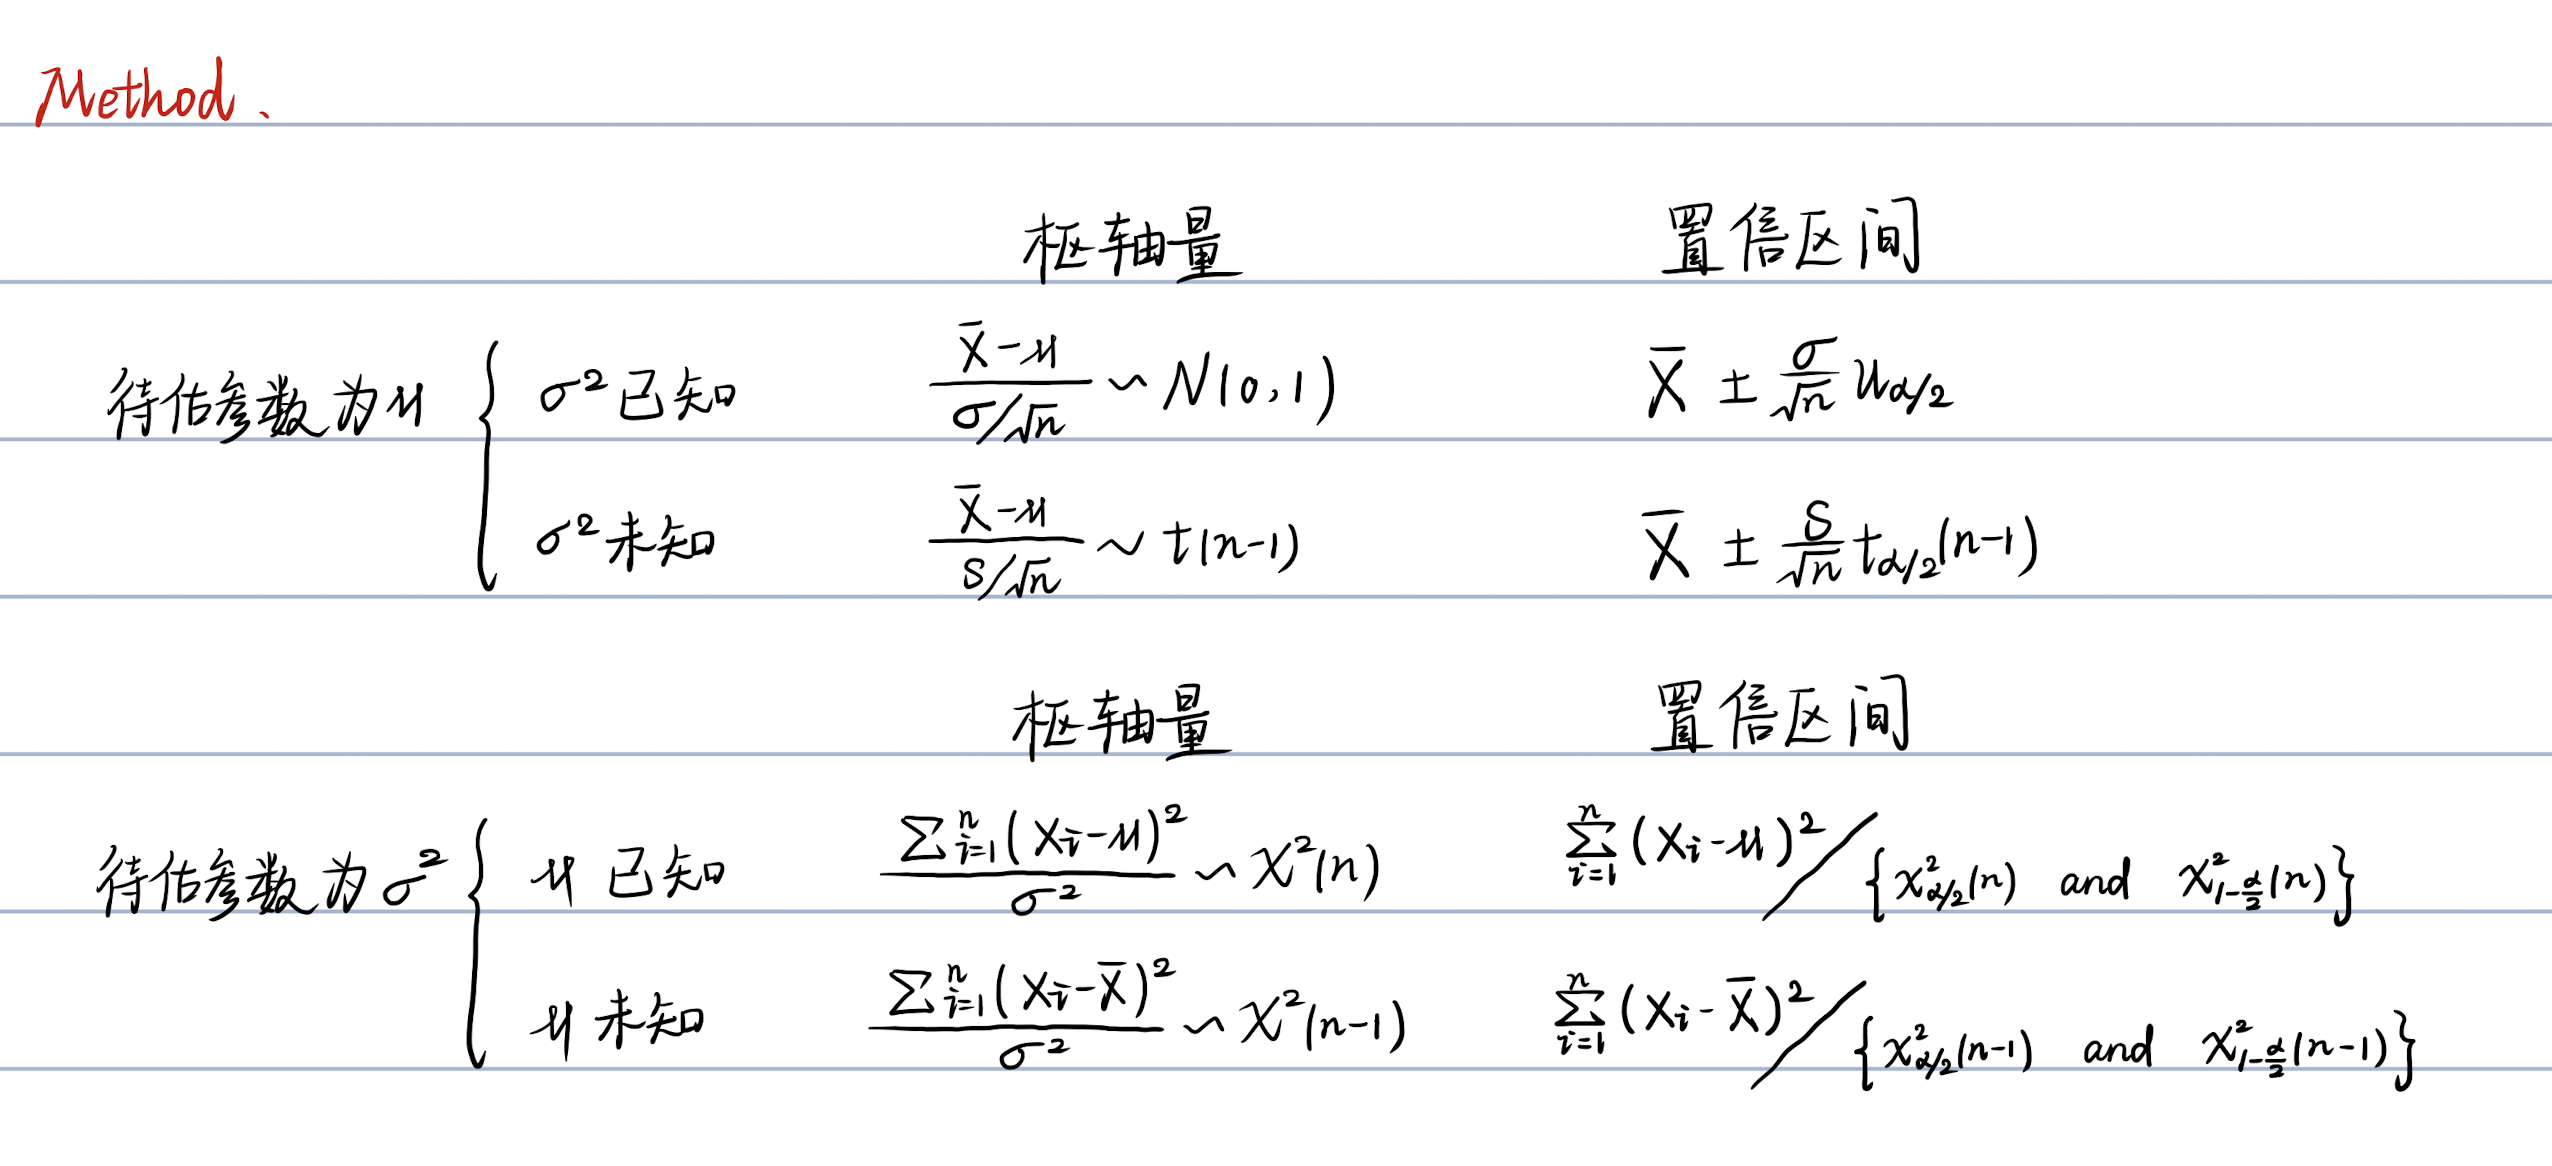
\includegraphics[width=0.82\linewidth]{N_confidence.png}
	\caption{单个正态总体参数的置信区间}
\end{figure}

\section{假设检验}
\begin{defi}[p值检验法]
    
\end{defi}
\textbf{\color{Red}一定要注意大于小于号!}

过程与置信区间一致,略。

\end{document}

